\documentclass[12pt,a4paper]{article}

\usepackage[margin=1in]{geometry}
\usepackage{array}
\usepackage{booktabs}
\usepackage{enumitem}
\usepackage{tikz}
\usetikzlibrary{arrows.meta,positioning,shapes.geometric}

\setlength{\parindent}{0pt}
\setlength{\parskip}{0.55em}
\renewcommand{\arraystretch}{1.22}
\newcolumntype{L}[1]{>{\raggedright\arraybackslash}p{#1}}

\title{\textbf{Deadlock Analysis and Prevention}}
\author{
  Name: \rule{7cm}{0.4pt}\\
  ID: \rule{7.5cm}{0.4pt}\\
  Course: Operating Systems
}
\date{}

\begin{document}
\maketitle

\section*{Given System State}

\begin{center}
\begin{tabular}{>{\bfseries}c L{5cm} L{4.5cm}}
\toprule
Process & Allocated Resource & Waiting For \\
\midrule
P1 & DB1 & PR1 \\
P2 & PR1 & BS1 \\
P3 & BS1 & DB2 \\
P4 & DB2 & DB1 \\
\bottomrule
\end{tabular}
\end{center}

Available resources: PR2 only. The analysis treats DB1, DB2, PR1, PR2, and BS1 as exact resource instances, because the question specifies exact resources in the waiting column.

\section*{1. Resource Allocation Graph}

\begin{center}
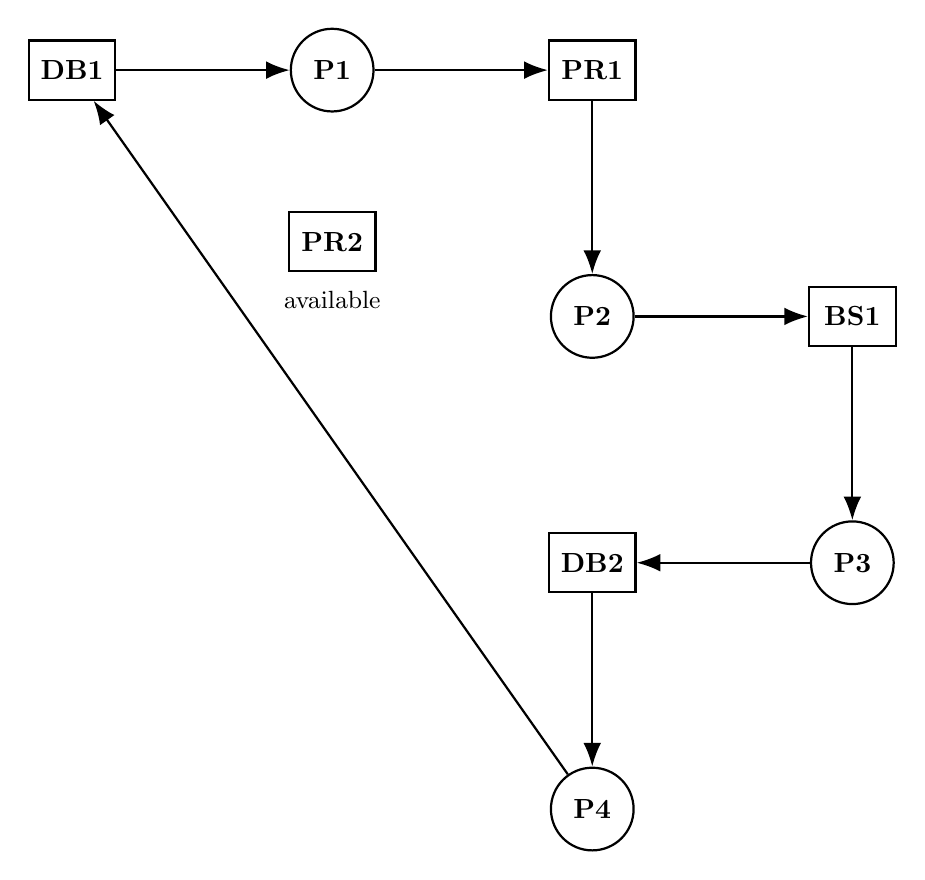
\begin{tikzpicture}[
  process/.style={circle, draw, thick, minimum size=1.05cm, font=\bfseries},
  resource/.style={rectangle, draw, thick, minimum width=1.1cm, minimum height=0.75cm, font=\bfseries},
  edge/.style={-{Latex[length=3mm]}, thick},
  node distance=2.2cm
]
  \node[process] (p1) {P1};
  \node[resource, right=of p1] (pr1) {PR1};
  \node[process, below=of pr1] (p2) {P2};
  \node[resource, right=of p2] (bs1) {BS1};
  \node[process, below=of bs1] (p3) {P3};
  \node[resource, left=of p3] (db2) {DB2};
  \node[process, below=of db2] (p4) {P4};
  \node[resource, left=of p1] (db1) {DB1};
  \node[resource, below=1.25cm of p1] (pr2) {PR2};

  \draw[edge] (db1) -- (p1);
  \draw[edge] (p1) -- (pr1);
  \draw[edge] (pr1) -- (p2);
  \draw[edge] (p2) -- (bs1);
  \draw[edge] (bs1) -- (p3);
  \draw[edge] (p3) -- (db2);
  \draw[edge] (db2) -- (p4);
  \draw[edge] (p4) -- (db1);

  \node[below=0.12cm of pr2, font=\small] {available};
\end{tikzpicture}
\end{center}

The cycle is:

\begin{center}
\textbf{P1 $\rightarrow$ PR1 $\rightarrow$ P2 $\rightarrow$ BS1 $\rightarrow$ P3 $\rightarrow$ DB2 $\rightarrow$ P4 $\rightarrow$ DB1 $\rightarrow$ P1}
\end{center}

\section*{2. Allocation, Request, and Available Vectors}

\begin{center}
\begin{tabular}{c c c c c c}
\toprule
\textbf{Allocation} & DB1 & DB2 & PR1 & PR2 & BS1 \\
\midrule
P1 & 1 & 0 & 0 & 0 & 0 \\
P2 & 0 & 0 & 1 & 0 & 0 \\
P3 & 0 & 0 & 0 & 0 & 1 \\
P4 & 0 & 1 & 0 & 0 & 0 \\
\bottomrule
\end{tabular}
\hspace{0.6cm}
\begin{tabular}{c c c c c c}
\toprule
\textbf{Request} & DB1 & DB2 & PR1 & PR2 & BS1 \\
\midrule
P1 & 0 & 0 & 1 & 0 & 0 \\
P2 & 0 & 0 & 0 & 0 & 1 \\
P3 & 0 & 1 & 0 & 0 & 0 \\
P4 & 1 & 0 & 0 & 0 & 0 \\
\bottomrule
\end{tabular}
\end{center}

\begin{center}
\begin{tabular}{c c c c c}
\toprule
\textbf{Available DB1} & \textbf{DB2} & \textbf{PR1} & \textbf{PR2} & \textbf{BS1} \\
\midrule
0 & 0 & 0 & 1 & 0 \\
\bottomrule
\end{tabular}
\end{center}

Only PR2 is available, but no process is waiting for PR2. Therefore no process can be chosen as the first process in a safe sequence.

\section*{3. Deadlock Analysis}

The waiting dependency is:

\begin{center}
\textbf{P1 waits for P2, P2 waits for P3, P3 waits for P4, and P4 waits for P1.}
\end{center}

\begin{center}
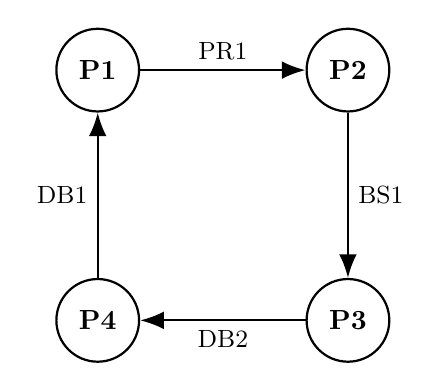
\begin{tikzpicture}[
  process/.style={circle, draw, thick, minimum size=1.05cm, font=\bfseries},
  edge/.style={-{Latex[length=3mm]}, thick},
  node distance=2.1cm
]
  \node[process] (p1) {P1};
  \node[process, right=of p1] (p2) {P2};
  \node[process, below=of p2] (p3) {P3};
  \node[process, below=of p1] (p4) {P4};

  \draw[edge] (p1) -- node[above, font=\small] {PR1} (p2);
  \draw[edge] (p2) -- node[right, font=\small] {BS1} (p3);
  \draw[edge] (p3) -- node[below, font=\small] {DB2} (p4);
  \draw[edge] (p4) -- node[left, font=\small] {DB1} (p1);
\end{tikzpicture}
\end{center}

This wait-for graph has the cycle P1 $\rightarrow$ P2 $\rightarrow$ P3 $\rightarrow$ P4 $\rightarrow$ P1. Since no process releases its allocated resource while waiting, none of them can complete. Hence, the system is \textbf{deadlocked}.

\section*{4. Four Necessary Conditions}

\begin{center}
\begin{tabular}{L{3.5cm} L{10cm}}
\toprule
\textbf{Condition} & \textbf{How it appears in this case} \\
\midrule
Mutual exclusion & DB1, DB2, PR1, PR2, and BS1 are limited resources assigned to one process at a time. \\
Hold and wait & Each process holds one resource while waiting for another resource. \\
No preemption & The problem states that no process releases its allocated resource while waiting. \\
Circular wait & P1 waits for P2, P2 waits for P3, P3 waits for P4, and P4 waits for P1. \\
\bottomrule
\end{tabular}
\end{center}

All four conditions hold simultaneously, so deadlock is confirmed.

\section*{5. Prevention and Avoidance}

\begin{center}
\begin{tabular}{L{3.5cm} L{5.2cm} L{5.2cm}}
\toprule
\textbf{Method} & \textbf{Use} & \textbf{Limitation} \\
\midrule
Request all resources at once & Prevents hold-and-wait. & Low resource utilization. \\
Resource ordering & Prevents circular wait by forcing a fixed request order. & All programs must follow the same rule. \\
Preemption and rollback & Recovers resources from blocked processes. & Hard for printer, database, and backup operations. \\
Banker's algorithm & Grants a request only if the state remains safe. & Needs maximum demand information in advance. \\
Timeout and retry & Detects long waits and restarts affected processes. & Recovery technique, not full prevention. \\
\bottomrule
\end{tabular}
\end{center}

\section*{6. Recommendation}

The best practical solution is \textbf{resource ordering}, supported by timeout-based rollback. A suitable global order is:

\begin{center}
\textbf{Database connections $\rightarrow$ Printers $\rightarrow$ Backup storage}
\end{center}

Each process must request resources only in this order. This directly prevents circular wait, which is the main cause of the observed deadlock. Timeout and rollback should also be used so that abnormal or long-waiting processes release resources and do not block the server indefinitely.

\section*{Conclusion}

The system is deadlocked because the resource allocation graph and wait-for graph both contain a cycle, and no process can start a safe completion sequence. The most suitable solution is to enforce a fixed resource-ordering policy with timeout-based recovery.

\end{document}
